\documentclass[13pt,a4paper]{extarticle}
% =========================================================
% FONT CHU - TOAN BO BAO CAO DUNG TIMES NEW ROMAN
% =========================================================
\usepackage{fontspec}
% Ưu tiên Times New Roman; dùng font cùng họ Times nếu máy biên dịch chưa có TNR.
\IfFontExistsTF{Times New Roman}{%
    \setmainfont{Times New Roman}
    \setsansfont{Times New Roman}
    \setmonofont{Times New Roman}
}{%
    \setmainfont{TeX Gyre Termes}
    \setsansfont{TeX Gyre Termes}
    \setmonofont{TeX Gyre Termes}
}
% =========================================================
% THU VIEN
% =========================================================
\usepackage{geometry}
\usepackage{tikz}
\usetikzlibrary{
    arrows.meta,
    positioning,
    shapes.geometric,
    fit,
    calc
}
\usepackage{graphicx}
% Biên dịch tại ketqua/ hoặc từ thư mục package đều tìm được các ảnh có sẵn.
\graphicspath{{./}{ketqua/}{images/}}
\usepackage{array}
\usepackage{float}
\usepackage{tabularx}
\usepackage{booktabs}
\usepackage{amsmath}
\usepackage{fancyvrb}
\usepackage{xcolor}
\usepackage{xurl}
% --- them cho phan noi dung ---
\usepackage{caption}
\usepackage{subcaption}
\usepackage{enumitem}
\usepackage{setspace}
\usepackage{longtable}
\usepackage{needspace} % Tránh để tiêu đề mục cây thư mục nằm lẻ cuối trang.
% =========================================================
% CAN LE
% =========================================================
\geometry{
    top=2cm,
    bottom=2cm,
    left=2cm,
    right=2cm
}
% =========================================================
% LINK
% =========================================================
\usepackage[
    colorlinks=true,
    linkcolor=black,
    urlcolor=blue,
    citecolor=black
]{hyperref}
% =========================================================
% CAC LENH DUNG TRONG NOI DUNG
% =========================================================
% Ten file, node, topic, package...
% Van dung Times New Roman, khong chuyen sang font monospace
\urlstyle{rm}
% \code: cho phep xuong dong giua ten dai (khong dung duoc trong \caption va khi co dau cach)
\newcommand{\code}[1]{%
    \path{#1}%
}
% \cmd: giong \code cu cua ban (khong xuong dong, giu dau cach, dung duoc trong \caption)
\newcommand{\cmd}[1]{%
    \textnormal{\detokenize{#1}}%
}
\newcommand{\codeb}[1]{%
    \textnormal{\detokenize{#1}}%
}
% Ghi chu
\newcommand{\todo}[1]{%
    \textit{#1}%
}
% Khung cho anh
\newcommand{\placeholderfig}[2]{%
    \begin{figure}[H]
        \centering
        \fbox{%
            \parbox[c][#1][c]{0.88\linewidth}{%
                \centering
                #2
            }%
        }
    \end{figure}%
}
% Chen hinh: co file trong images/ thi hien anh, chua co thi hien khung trong
\newcommand{\hinh}[3]{%
  \begin{figure}[H]\centering
  \IfFileExists{images/#1}%
    {\includegraphics[width=#2\textwidth]{images/#1}}%
    {\IfFileExists{ketqua/#1}%
      {\includegraphics[width=#2\textwidth]{ketqua/#1}}%
      {\fbox{\parbox{0.8\textwidth}{\centering\vspace{2.2cm}\textit{[Chèn ảnh \detokenize{#1}]}\vspace{2.2cm}}}}}%
  \caption{#3}
  \end{figure}}

% Ảnh bổ sung: tự hiển thị khi có file; chưa có thì giữ khung mô tả cần chụp gì.
% #1 tên ảnh, #2 phần chiều rộng trang, #3 chiều cao khung chờ,
% #4 nội dung khung, #5 chú thích, #6 nhãn tham chiếu.
\newcommand{\reportimage}[6]{%
  \begin{figure}[H]
  \centering
  \IfFileExists{#1}%
    {\includegraphics[width=#2\textwidth]{#1}}%
    {\IfFileExists{ketqua/#1}%
      {\includegraphics[width=#2\textwidth]{ketqua/#1}}%
      {\IfFileExists{images/#1}%
        {\includegraphics[width=#2\textwidth]{images/#1}}%
        {\fbox{\parbox[c][#3][c]{0.84\linewidth}{\centering\small\itshape #4}}}}}%
  \caption{#5}
  \label{#6}
  \end{figure}%
}

% Nhánh cây dùng ký tự văn bản có sẵn trong font Times, không cần font vẽ khung.
% #1 mức thụt lề tính bằng em; #2 tên thư mục/file, kể cả dấu gạch dưới.
\newcommand{\treeentry}[2]{%
    \hspace*{#1em}\textbar\kern0.1em\textendash\kern0.35em\cmd{#2}%
}

% Vai trò của file con thụt vào cùng cấp với tên file ở cột trái.
% leftskip giữ cả các dòng xuống hàng thẳng theo lề mới, không chỉ dòng đầu.
\newcommand{\treerole}[2]{%
    \begingroup
    \setlength{\leftskip}{#1em}%
    \noindent\# #2\par
    \endgroup
}

\newcolumntype{L}[1]{>{\raggedright\arraybackslash}p{#1}}
\newcolumntype{Y}{>{\raggedright\arraybackslash}X}
\renewcommand{\figurename}{Hình}
\renewcommand{\tablename}{Bảng}
\captionsetup{font=small,labelfont=bf}
\setstretch{1.15}
\setlength{\parindent}{1.2em}
\setlength{\parskip}{2pt}
\setlist{itemsep=1pt,topsep=3pt}
\emergencystretch=3em
% =========================================================
% VERBATIM CUNG DUNG TIMES NEW ROMAN
% =========================================================
\DefineVerbatimEnvironment{Verbatim}{Verbatim}{
    fontfamily=\rmdefault
}
% =========================================================
% TRANG BIA KHONG DANH SO TRANG
% =========================================================
\pagestyle{empty}
\usepackage{placeins}
\begin{document}

% ==================== KHUNG BIA ====================
\begin{tikzpicture}[remember picture,overlay]

% Khung ngoai mong
\draw[
    blue!50!black,
    line width=0.8pt
]
([xshift=1.65cm,yshift=-1.45cm]current page.north west)
rectangle
([xshift=-1.65cm,yshift=1.45cm]current page.south east);

% Khung trong dam
\draw[
    blue!70!black,
    line width=3pt
]
([xshift=1.85cm,yshift=-1.65cm]current page.north west)
rectangle
([xshift=-1.85cm,yshift=1.65cm]current page.south east);

\end{tikzpicture}


% ==================== NOI DUNG BIA ====================

\begin{center}

\vspace*{0.7cm}

{\bfseries\fontsize{16}{20}\selectfont
TRƯỜNG ĐẠI HỌC CÔNG NGHỆ
\par}

\vspace{0.25cm}

{\bfseries\fontsize{16}{20}\selectfont
ĐẠI HỌC QUỐC GIA HÀ NỘI
\par}


% ==================== LOGO ====================

\vspace{1.5cm}

% Giữ vị trí logo; chưa có file thì vẫn biên dịch được báo cáo.
\IfFileExists{logo-uet.png}{%
    \includegraphics[width=5.3cm]{logo-uet.png}%
}{%
    \IfFileExists{ketqua/logo-uet.png}{%
        \includegraphics[width=5.3cm]{ketqua/logo-uet.png}%
    }{%
        \fbox{\parbox[c][3.6cm][c]{5.0cm}{\centering
        \bfseries UET\\[0.4cm]
        \normalfont\small Bổ sung logo trường\\
        \cmd{logo-uet.png}}}%
    }%
}

\vspace{1.5cm}


% ==================== TEN BAO CAO ====================

{\bfseries\fontsize{16}{20}\selectfont
BÁO CÁO THỰC HÀNH 7
\par}

\vspace{0.45cm}
{\bfseries\fontsize{15}{19}\selectfont
PHÂN VÙNG BẢN ĐỒ VÀ ĐIỀU HƯỚNG\\
TURTLEBOT 4 BẰNG GIỌNG NÓI
\par}


\end{center}


\vspace{1.8cm}



% ==================== GIANG VIEN ====================

\noindent
\hspace*{2cm}%
\begin{tabular}{
    @{}
    >{\bfseries}p{5cm}
    p{7cm}
    @{}
}
Giảng viên phụ trách:
&
\textbf{PGS.TS Hoàng Văn Xiêm}
\\
&
\textbf{HVCH Nguyễn Quốc Bảo}\\
\end{tabular}

\vspace{2cm}

% ==================== SINH VIEN ====================

\noindent
\hspace*{2cm}%
\begin{tabular}{
    @{}
    >{\bfseries}p{5cm}
    p{7cm}
    @{}
}
Sinh viên thực hiện:
&
\textbf{Văn Thư Đạt -- 23020733}
\end{tabular}


% =================================================
%                     MỤC LỤC
% =================================================

\newpage
\pagestyle{plain}

% Hiển thị:
% section    = mục lớn
% subsection = mục con
% Không hiển thị subsubsection
\setcounter{tocdepth}{2}

\begin{center}
    {\bfseries\Large MỤC LỤC}
\end{center}

\vspace{0.4cm}

\begingroup
\small
\setlength{\parskip}{0pt}

\makeatletter
\@starttoc{toc}
\makeatother

\endgroup

\newpage

% ==================================================
%                   NOI DUNG BAO CAO
% ==================================================

\Needspace{17cm}
\section{Kiến trúc hệ thống}

\subsection{Sơ đồ tổng thể}

Bài thực hành 7 tập trung xây dựng hệ thống phân vùng bản đồ và điều hướng TurtleBot 4 bằng giọng nói tiếng Việt trên Ubuntu 22.04, ROS 2 Humble và Gazebo Fortress. Hệ thống tiếp nhận câu lệnh, chuyển âm thanh thành văn bản, xác định thứ tự các khu vực cần đến và gửi mục tiêu cho Nav2. Bản đồ được chia thành năm vùng chức năng: phòng ngủ, phòng sinh hoạt, hành lang, phòng khách và nhà bếp. Trong phạm vi bài thực hành, ranh giới các vùng được xác định bằng đa giác (polygon) thủ công, kết hợp xử lý ảnh để gán nhãn và lựa chọn điểm đích.

\begin{figure}[H]
\centering
\resizebox{0.98\linewidth}{!}{%
\begin{tikzpicture}[
    base/.style={rounded corners=3pt,align=center,text width=4.4cm,
                 inner sep=6pt,minimum height=2.8cm,
                 font=\fontsize{10.5}{12.5}\selectfont},
    rosnode/.style={base,draw=blue!65!black,fill=blue!6,line width=0.8pt},
    topic/.style={base,draw=orange!80!black,fill=yellow!16,line width=0.8pt},
    device/.style={base,draw=black!60,fill=black!4,line width=0.8pt},
    execution/.style={base,draw=green!45!black,fill=green!6,line width=0.8pt},
    data/.style={-{Latex[length=2.2mm]},thick,draw=blue!65!black},
    command/.style={-{Latex[length=2.2mm]},thick,draw=green!40!black},
    feedback/.style={-{Latex[length=2.2mm]},thick,dashed,draw=orange!75!black},
    note/.style={font=\fontsize{9}{11}\selectfont,fill=white,
                 inner sep=3pt,align=center}
]
% Khối có cùng chiều cao; khoảng trống riêng cho dây và nhãn.
\node[device] (microphone) at (0,0)
    {\textbf{MICROPHONE}\\Âm thanh tiếng Việt\\Thu mono, chuẩn hóa 16 kHz};
\node[rosnode] (speech) at (7,0)
    {\textbf{NODE GIỌNG NÓI}\\\cmd{speech_node}\\Thu/VAD và giải mã riêng\\PhoWhisper-small, CPU int8};
\node[topic] (text) at (14,0)
    {\textbf{VĂN BẢN ĐÃ NHẬN}\\\cmd{/voice_navigation/speech}\\\cmd{std_msgs/msg/String}\\JSON: câu nói và thời điểm thu};
\node[device] (map) at (0,-5.4)
    {\textbf{BẢN ĐỒ VÀ KHU VỰC}\\\cmd{map.pgm}, \cmd{map.yaml}\\OpenCV + polygon thủ công\\\cmd{regions.yaml}: ID, tên, goal};
\node[execution] (nav2) at (7,-5.4)
    {\textbf{NAV2}\\Action \cmd{/navigate_to_pose}\\AMCL, costmap, lập đường\\Điều khiển tránh vật cản};
\node[rosnode] (navigation) at (14,-5.4)
    {\textbf{NODE ĐIỀU HƯỚNG}\\\cmd{voice_navigation_node}\\Phân tích mẫu câu, tra tên vùng\\Gửi lần lượt các goal};
\node[device] (robot) at (0,-10.8)
    {\textbf{TURTLEBOT 4 / GAZEBO}\\Thực thi chuyển động\\Cung cấp LiDAR, odometry, TF};
\node[topic] (status) at (7,-10.8)
    {\textbf{TRẠNG THÁI TUYẾN}\\\cmd{/voice_navigation/status}\\\cmd{std_msgs/msg/String}\\Tuyến, chặng, kết quả, kết nối};
\node[execution] (gui) at (14,-10.8)
    {\textbf{GIAO DIỆN / RVIZ}\\Khu vực, vị trí, đường Nav2\\Hiển thị câu nhận dạng\\Gửi lệnh và yêu cầu dừng};

% Luồng chính: nhãn nằm trong khe giữa các khối.
\draw[data] (microphone.east) -- node[note,above=2pt] {PCM} (speech.west);
\draw[data] (speech.east) -- node[note,above=2pt] {publish} (text.west);
\draw[data] (text.south) -- node[note,right=3pt] {subscribe} (navigation.north);
\draw[data] (map.east) -- node[note,above=2pt] {map} (nav2.west);
\draw[command] (navigation.west) -- node[note,above=2pt] {goal / hủy} (nav2.east);

% Dữ liệu khu vực đi ở hành lang phía trên hàng giữa.
\draw[data] (map.north) -- (0,-2.7)
    -- node[note,above=2pt] {ID, tên vùng và tọa độ goal} (12.8,-2.7)
    -- ([xshift=-1.2cm]navigation.north);

% Hai chiều giữa Nav2 và robot được gom trên một đường, tránh dây chéo nhau.
\draw[command,<->] (nav2.south west)
    -- node[note,above=4pt] {Vận tốc / controller\\LiDAR, odometry, TF} (robot.north east);

% Hai kênh riêng: kết quả action ở trên, trạng thái GUI ở dưới.
\draw[feedback] ([xshift=1.2cm]nav2.south) -- (8.2,-7.7)
    -- node[note,above=2pt] {Kết quả goal} (12.8,-7.7)
    -- ([xshift=-1.2cm]navigation.south);
\draw[feedback] ([xshift=1.2cm]navigation.south) -- (15.2,-8.5)
    -- node[note,below=2pt] {Trạng thái tuyến} (7,-8.5)
    -- (status.north);
\draw[feedback] (status.east) -- node[note,above=2pt] {subscribe} (gui.west);

% Lệnh từ GUI vòng bên ngoài, không đi qua nội dung các khối.
\draw[command] (gui.east) -- (18.3,-10.8)
    -- node[note,left=3pt] {Lệnh\\GUI} (18.3,-5.4)
    -- (navigation.east);
\node[note,anchor=north,text width=18cm] at (7,-13.1)
    {Vận tốc đi từ Nav2 tới robot; dữ liệu cảm biến và TF phản hồi về Nav2.\\
     GUI đọc thêm \cmd{/amcl_pose}, \cmd{/plan}; RViz đọc map, TF, scan, costmap và marker vùng.};
\end{tikzpicture}%
}
\caption{Kiến trúc phân vùng bản đồ, nhận giọng nói và điều hướng qua Nav2.}
\label{fig:architecture}
\end{figure}

\Needspace{4\baselineskip}
\noindent\begin{minipage}{\linewidth}
\section{Tổ chức mã nguồn và luồng dữ liệu}
\subsection{Cây thư mục}

Mã nguồn được tổ chức thành package ROS 2 \code{tb4_voice_navigation}, gồm các module xử lý bản đồ, nhận dạng giọng nói, phân tích câu lệnh và điều hướng. Cách tổ chức này giúp kiểm tra từng khâu và thuận tiện khi mở rộng chức năng. Các node cùng sử dụng dữ liệu khu vực trong file YAML để thống nhất tên phòng và tọa độ đích.

\par\vspace{6pt}
\begingroup
\fontsize{10.5}{12.5}\selectfont
\setstretch{1.0}
\renewcommand{\arraystretch}{1.03}
\setlength{\aboverulesep}{4pt}
\setlength{\belowrulesep}{4pt}
\noindent\begin{tabular}{@{}L{0.38\linewidth}L{0.58\linewidth}@{}}
\toprule
\textbf{Thư mục / file} & \textbf{Vai trò trong dự án} \\
\midrule
\cmd{tb4_voice_navigation/} & \# Package phân vùng và điều hướng giọng nói. \\
\treeentry{0}{launch/} & \# Các cấu hình khởi chạy hệ thống. \\
\treeentry{1.2}{building_sim.launch.py} & \treerole{1.2}{Mở căn nhà, robot, dock và bridge.} \\
\treeentry{1.2}{building_mapping.launch.py} & \treerole{1.2}{Quét map khi cần bằng SLAM Toolbox.} \\
\treeentry{1.2}{building_navigation.launch.py} & \treerole{1.2}{Mở mô phỏng, map đã lưu, AMCL, Nav2, RViz.} \\
\treeentry{1.2}{voice_navigation.launch.py} & \treerole{1.2}{Chạy nhận giọng nói, điều hướng và giao diện.} \\
\treeentry{0}{config/} & \# Tham số phân vùng và điều hướng. \\
\treeentry{1.2}{region_definitions.yaml} & \treerole{1.2}{Polygon, tên vùng và điểm đích mong muốn.} \\
\treeentry{1.2}{nav2.yaml} & \treerole{1.2}{Planner, controller, costmap và ngưỡng đến đích.} \\
\treeentry{1.2}{localization.yaml} & \treerole{1.2}{Tham số định vị AMCL.} \\
\treeentry{1.2}{slam.yaml} & \treerole{1.2}{Tham số khi cần tạo bản đồ mới.} \\
\treeentry{0}{maps/} & \# Bản đồ và dữ liệu ngữ nghĩa. \\
\treeentry{1.2}{map.pgm, map.yaml} & \treerole{1.2}{Ảnh Occupancy Grid, độ phân giải và gốc tọa độ.} \\
\treeentry{1.2}{regions.yaml} & \treerole{1.2}{ID, tên, alias, polygon và tọa độ goal.} \\
\treeentry{1.2}{segmented_map.png} & \treerole{1.2}{Ảnh màu các vùng và chú giải.} \\
\treeentry{1.2}{region_labels.png} & \treerole{1.2}{Ảnh mã vùng 0--5 dùng cho chương trình.} \\
\treeentry{0}{tb4_voice_navigation/} & \# Các module Python của package. \\
\treeentry{1.2}{map_tools.py, segment_map.py} & \treerole{1.2}{Đọc map, đổi tọa độ, tạo nhãn và chọn đích.} \\
\treeentry{1.2}{audio_capture.py} & \treerole{1.2}{Thu âm, VAD và giải mã trong worker riêng.} \\
\treeentry{1.2}{speech_node.py} & \treerole{1.2}{Điều khiển mic, publish câu nhận dạng và trạng thái.} \\
\treeentry{1.2}{voice_model.py} & \treerole{1.2}{Tải PhoWhisper và chuyển sang CTranslate2 int8.} \\
\treeentry{1.2}{commands.py} & \treerole{1.2}{Chuẩn hóa chữ, kiểm tra tên và tạo tuyến.} \\
\treeentry{1.2}{navigation_node.py} & \treerole{1.2}{Gửi goal Nav2, theo dõi kết quả và hủy tuyến.} \\
\treeentry{1.2}{voice_control_gui.py} & \treerole{1.2}{Hiển thị map, câu nói, đường đi và tiến độ.} \\
\treeentry{0}{worlds/, models/, rviz/} & \# Môi trường 3D, nội thất và cấu hình hiển thị. \\
\treeentry{0}{ketqua/} & \# Ảnh thực nghiệm và mã nguồn báo cáo. \\
\treeentry{0}{resource/, package.xml} & \# Đăng ký package và khai báo phụ thuộc ROS. \\
\treeentry{0}{setup.py, setup.cfg} & \# Cài module, tài nguyên và các executable. \\
\treeentry{0}{requirements.txt, README.md} & \# Thư viện Python và hướng dẫn sử dụng. \\
\bottomrule
\end{tabular}
\par\endgroup
\vspace{6pt}

Trọng số mô hình được lưu trong bộ nhớ đệm (cache) của người dùng, tách khỏi mã nguồn. Thư mục \code{ketqua/} chứa ảnh thực nghiệm và báo cáo.
\end{minipage}
\par\medskip

\subsection{Các node và luồng dữ liệu}

Luồng xử lý của hệ thống được trình bày trong Hình~\ref{fig:architecture}. Dữ liệu và trạng thái được trao đổi qua topic; service được sử dụng để bật/tắt microphone; action được sử dụng để gửi mục tiêu điều hướng, nhận phản hồi và hủy mục tiêu khi cần.

\begin{enumerate}[label=\arabic*.,leftmargin=1.6em,itemsep=5pt]
\item \textbf{Chuẩn bị bản đồ và khởi chạy mô phỏng.} Hệ thống sử dụng môi trường mô phỏng TurtleBot 4~\hyperref[ref:tb4sim]{[5]} và bản đồ SLAM có sẵn. Bản đồ được xử lý bằng OpenCV và gắn nhãn theo các polygon đã khai báo. File \code{building_navigation.launch.py} khởi chạy Gazebo, map server, AMCL, Nav2 và RViz. Robot được đưa ra khỏi dock bằng thao tác Undock trước khi nhận mục tiêu. Chức năng tạo bản đồ mới được cấu hình trong launch riêng để tách quá trình SLAM khỏi chế độ định vị trên bản đồ đã lưu.
\item \textbf{Thu âm và chuyển thành văn bản.} Node \code{speech_node} điều khiển một worker riêng. Worker thu âm, tìm đoạn có tiếng nói và dùng PhoWhisper-small để nhận dạng tiếng Việt. Kết quả hoàn chỉnh được gửi trên \code{/voice_navigation/speech}, kèm thời điểm thu để phát hiện câu quá cũ. Việc giải mã không chạy trong callback ROS.
\item \textbf{Phân tích yêu cầu và kiểm tra tên khu vực.} Node \code{voice_navigation_node} gọi \code{parse_command()} trong \code{commands.py}. Văn bản được chuyển về chữ thường, bỏ dấu và dấu câu để tra cứu tên/alias. Các mẫu ``đi đến'', ``di chuyển vào'', ``đi từ A qua C rồi đến B'' được đổi thành danh sách ID. Tất cả tên phải hợp lệ trước khi có bất kỳ goal nào được gửi.
\item \textbf{Thực hiện từng mục tiêu Nav2.} Node tạo \code{PoseStamped} trong frame \code{map}, chuyển góc yaw sang quaternion và gửi action \code{NavigateToPose}. Nav2 phụ trách lập đường và tránh vật cản. Khi chặng hiện tại thành công, node mới tăng chỉ số và gửi chặng kế tiếp; chặng thất bại thì kết thúc tuyến. Module giọng nói không tự phát vận tốc để thay thế Nav2.
\item \textbf{Cập nhật giao diện và nhận yêu cầu dừng.} GUI PyQt5 hiển thị câu nhận dạng, các vùng, vị trí AMCL, đường \code{/plan} và số điểm đã hoàn thành. Các nút chọn phòng hoặc ô nhập chữ dùng chung bộ phân tích với giọng nói. Nút dừng gửi yêu cầu hủy goal; tắt microphone chỉ đóng thu âm, không tự hủy hành trình.
\end{enumerate}

\begin{table}[H]
\centering\small
\renewcommand{\arraystretch}{1.15}
\begin{tabularx}{\linewidth}{@{}L{4.0cm}L{4.6cm}Y@{}}
\toprule
\textbf{Topic / giao tiếp} & \textbf{Kiểu dữ liệu} & \textbf{Vai trò} \\
\midrule
\code{/voice_navigation/speech} & \code{std_msgs/msg/String} & JSON chứa câu nói hoàn chỉnh và timestamp. \\
\code{/voice_navigation/command} & \code{std_msgs/msg/String} & Lệnh từ GUI, bàn phím hoặc yêu cầu dừng. \\
\code{/voice_navigation/status} & \code{std_msgs/msg/String} & Tuyến, chỉ số chặng, trạng thái và kết nối Nav2. \\
\code{/voice_navigation/microphone_state} & \code{std_msgs/msg/String} & Trạng thái bật/tắt, thiết bị và trạng thái nhận âm. \\
\code{/voice_navigation/regions} & \code{visualization_msgs/msg/MarkerArray} & Nhãn khu vực trên RViz. \\
\code{/amcl_pose} & \code{geometry_msgs/msg/PoseWithCovarianceStamped} & Vị trí và hướng ước lượng để vẽ robot. \\
\code{/plan} & \code{nav_msgs/msg/Path} & Đường Nav2 của chặng hiện tại. \\
\code{/voice_navigation/set_listening} & \code{std_srvs/srv/SetBool} & Service bật/tắt microphone. \\
\code{/navigate_to_pose} & \code{nav2_msgs/action/NavigateToPose} & Action điều hướng tới từng goal. \\
\bottomrule
\end{tabularx}
\caption{Các giao tiếp chính trong hệ thống điều hướng bằng giọng nói.}
\label{tab:topics}
\end{table}

\Needspace{4\baselineskip}
\section{Ánh xạ khu vực, câu lệnh và điều hướng robot}

Mỗi khu vực được gán một mã định danh (ID), tên chức năng và điểm đích đại diện. Phòng khách và nhà bếp có phần không gian mở, do đó ranh giới vùng được xác định theo chức năng sử dụng, không chỉ dựa vào tường bao. Bảng~\ref{tab:regions} trình bày các điểm đích trong hệ tọa độ \code{map}.

\begin{table}[H]
\centering\small
\renewcommand{\arraystretch}{1.2}
\begin{tabularx}{\linewidth}{@{}L{0.7cm}L{3.1cm}L{3.0cm}L{1.5cm}Y@{}}
\toprule
\textbf{ID} & \textbf{Tên khu vực} & \textbf{Đích $(x;y)$, m} & \textbf{Yaw, rad} & \textbf{Khoảng hở trên map, m} \\
\midrule
A & Phòng ngủ & $(-5{,}945;\ 0{,}455)$ & $0$ & $0{,}60$ \\
B & Phòng sinh hoạt & $(-5{,}945;\ {-3{,}495})$ & $0$ & $0{,}90$ \\
C & Hành lang & $(-1{,}845;\ {-1{,}145})$ & $0$ & $1{,}00$ \\
D & Phòng khách & $(1{,}655;\ 0{,}205)$ & $0$ & $1{,}07$ \\
E & Nhà bếp & $(7{,}005;\ {-1{,}145})$ & $1{,}5708$ & $1{,}20$ \\
\bottomrule
\end{tabularx}
\caption{Năm khu vực và các điểm đích hợp lệ trên bản đồ.}
\label{tab:regions}
\end{table}

\subsection{Phân vùng bản đồ và gắn nhãn ngữ nghĩa}

\paragraph{Biểu diễn bản đồ ngữ nghĩa.}
Occupancy Grid biểu diễn không gian dưới dạng các ô trống, vật cản và vùng chưa biết, nhưng chưa chứa ý nghĩa như ``phòng ngủ'' hay ``nhà bếp''. Trong dự án, lớp ngữ nghĩa được bổ sung bằng tập khu vực $\mathcal{R}=\{R_A,R_B,R_C,R_D,R_E\}$. Mỗi khu vực lưu ID, tên, các tên gọi thay thế, polygon và tư thế đích $(x,y,\psi)$. Khi nhận câu lệnh, bộ phân tích tra cứu tên để tạo danh sách ID; node điều hướng dùng danh sách này để lấy tọa độ tương ứng. Cách biểu diễn trên tạo liên kết giữa tên khu vực trong ngôn ngữ và vị trí trên bản đồ. Nhãn được gán từ cấu hình, chưa được suy ra tự động từ ảnh nội thất hoặc dữ liệu cảm biến.


Bản đồ đầu vào \code{map.pgm} có kích thước $372\times221$ ô và độ phân giải $r=0{,}05$~m/ô. Với cấu hình \code{negate=0}, mức xám $I$ được chuyển thành giá trị chiếm chỗ $p=1-I/255$. Dựa trên ngưỡng \code{free_thresh} trong \code{map.yaml}, ô có $p<0{,}25$ được xác định là ô trống. Các ô vật cản và ô chưa biết được loại khỏi tập ứng viên khi chọn điểm đích.

Ranh giới từng khu vực được khai báo bằng polygon trong \code{region_definitions.yaml}. Chương trình chuyển tọa độ các đỉnh sang pixel, sử dụng \code{cv2.fillPoly()} để tạo mặt nạ vùng, sau đó lấy phần giao với tập ô trống. Nếu các polygon có phần biên chung, chương trình giữ nhãn đã gán trước để tránh ghi đè. Như vậy, phương pháp triển khai là phân vùng thủ công có hỗ trợ xử lý ảnh; các kỹ thuật tự động như watershed hoặc phép toán hình thái học (morphology) chưa được áp dụng trong phiên bản này.

\paragraph{Lựa chọn điểm đích đại diện.}
Tâm hình học của một vùng có thể nằm trên đồ vật hoặc gần tường, nên không thể sử dụng trực tiếp làm mục tiêu điều hướng. Chương trình dùng \code{cv2.distanceTransform()} để tính khoảng cách $d(q)$ từ ô trống $q$ tới ô không trống gần nhất, quy đổi sang mét~\hyperref[ref:opencv]{[1]}. Gọi $F$ là tập ô trống và $m=0{,}30$~m là khoảng hở tối thiểu. Tập ô thỏa mãn điều kiện khoảng hở được xác định bởi:
\begin{equation}
 F_m=\{q\in F\mid d(q)\geq m\}.
\end{equation}
Từ $F_m$, hàm \code{connectedComponents()} với kết nối bốn hướng giữ lại thành phần $C_s$ chứa điểm xuất phát cấu hình $(-0{,}6;0)$. Kết nối bốn hướng giúp loại trường hợp các ô chỉ tiếp xúc chéo tại góc. Với $P_i$ là tập ô thuộc polygon thứ $i$ sau khi xử lý biên chung, tập ứng viên của vùng là $G_i=P_i\cap C_s$. Nếu $q_i^{\mathrm{pref}}$ là pixel tương ứng với điểm đích mong muốn, chương trình chọn:
\begin{equation}
 q_i^*=\operatorname*{arg\,min}_{q\in G_i}
       \left\|q-q_i^{\mathrm{pref}}\right\|_2^2.
 \label{eq:region-goal}
\end{equation}
Đây là phép chọn ô hợp lệ gần điểm mong muốn nhất trong hệ tọa độ pixel, đúng với bước tìm cực tiểu trong \code{segment_map.py}. Nếu $G_i$ rỗng, chương trình báo lỗi và yêu cầu điều chỉnh vùng hoặc cấu hình khoảng hở. Ô được chọn được đổi sang tọa độ mét trước khi lưu vào YAML; góc hướng được lấy từ cấu hình.

Các điểm mong muốn hiện được đặt gần tâm từng vùng; riêng phòng ngủ dịch khỏi tâm khoảng 0,40~m để tránh mép giường. Các điểm đích sau xử lý có khoảng hở từ 0,60~m trở lên, lớn hơn ngưỡng tối thiểu $m$. Điều kiện liên thông và khoảng hở là kiểm tra trên ảnh lưới; khả năng thực hiện quỹ đạo còn được Nav2 kiểm tra theo mô hình robot và dữ liệu cảm biến trong quá trình di chuyển.

Kết quả xử lý gồm ảnh màu \code{segmented_map.png}, ảnh mã vùng \code{region_labels.png} và file \code{regions.yaml}. File YAML lưu ID, tên, tên gọi thay thế (alias), polygon, tọa độ đích và khoảng hở tương ứng. Ảnh mã vùng lưu giá trị từ 0 đến 5 để chương trình tra cứu; ảnh màu được sử dụng để trực quan hóa kết quả như Hình~\ref{fig:segmentation}.

\begin{figure}[H]
\centering
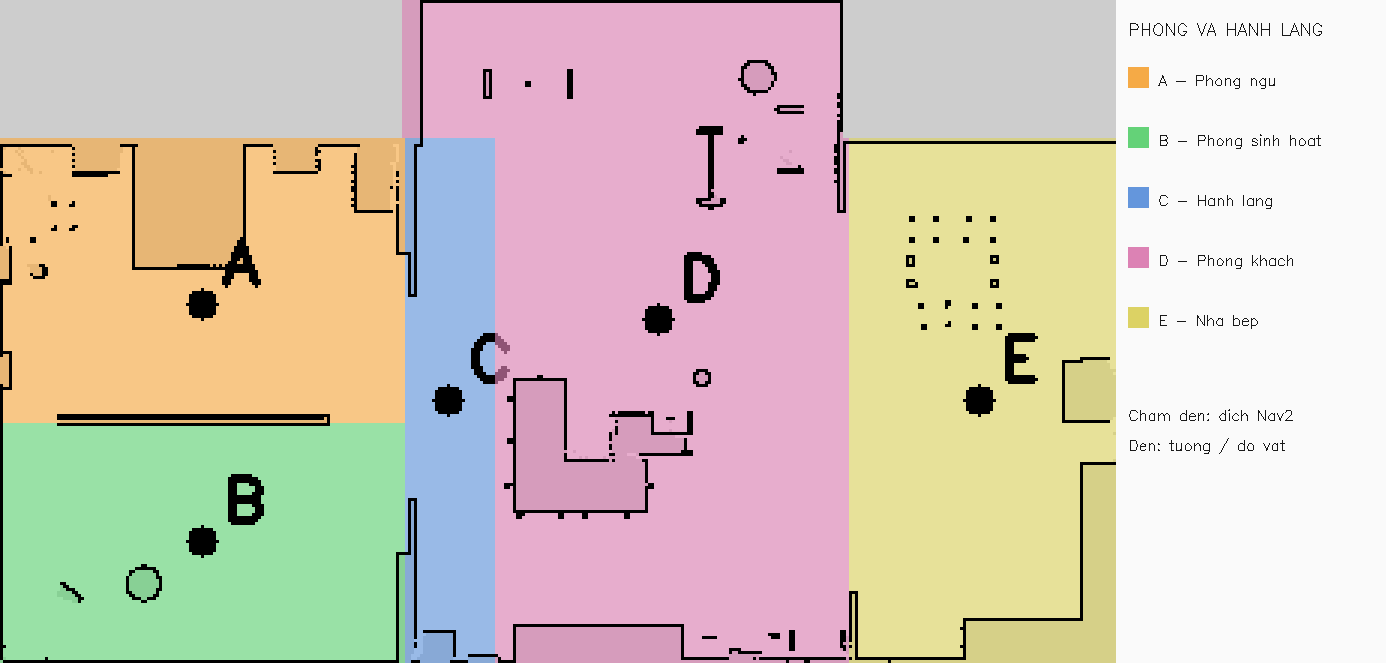
\includegraphics[width=0.98\linewidth]{segmented_map.png}
\caption{Bản đồ được phân thành năm khu vực A--E; chấm đen biểu thị các điểm đích đại diện.}
\label{fig:segmentation}
\end{figure}

\subsection{Nhận dạng giọng nói và phân tích yêu cầu}

\paragraph{Bài toán nhận dạng và lựa chọn mô hình.}
Nhận dạng giọng nói tự động (Automatic Speech Recognition -- ASR) là quá trình chuyển tín hiệu âm thanh thu từ microphone thành văn bản tiếng Việt. Chất lượng nhận dạng ảnh hưởng trực tiếp tới việc xác định tên phòng và thứ tự các điểm đến. Ví dụ, khi từ ``ngủ'' bị nhận dạng sai, hệ thống có thể từ chối câu lệnh dù đã nhận đúng cụm ``đi đến''. Vì vậy, khâu nhận dạng âm thanh và khâu phân tích câu lệnh được triển khai độc lập để thuận tiện xác định nguyên nhân lỗi.

Trong bài thực hành, em lựa chọn \code{vinai/PhoWhisper-small}, một mô hình được tinh chỉnh từ Whisper cho tiếng Việt. Theo công bố của nhóm tác giả, PhoWhisper được tinh chỉnh trên 844 giờ âm thanh với nhiều giọng vùng miền; phiên bản small có khoảng 244 triệu tham số~\hyperref[ref:phowhisper]{[2]}. Đặc điểm này phù hợp với yêu cầu nhận dạng câu lệnh tiếng Việt của dự án. Hệ thống sử dụng trọng số đã được huấn luyện sẵn để suy luận, chưa thực hiện huấn luyện hoặc tinh chỉnh trên dữ liệu giọng nói riêng.

\paragraph{Nguyên lý chuyển âm thanh thành văn bản.}
PhoWhisper kế thừa kiến trúc Transformer encoder--decoder của Whisper. Encoder tạo biểu diễn đặc trưng từ âm thanh; decoder sử dụng biểu diễn này và các token đã sinh để dự đoán token tiếp theo~\hyperref[ref:whisper]{[6]}. Token là đơn vị mã hóa của bộ từ vựng, có thể là một phần của từ, dấu câu hoặc token đặc biệt, không nhất thiết tương ứng một từ tiếng Việt hoàn chỉnh. Cơ chế attention cho phép kết hợp thông tin ở nhiều thời điểm thay vì phân loại từng âm hoặc từng từ một cách độc lập.

Trước khi đưa vào encoder, tín hiệu âm thanh dạng sóng (waveform) được biến đổi thành phổ log-Mel. Với cấu hình hiện tại, thư viện trích xuất 80 dải Mel từ tín hiệu 16~kHz, sử dụng cửa sổ 400 mẫu (25~ms) và bước dịch 160 mẫu (10~ms). Biểu diễn này mô tả sự thay đổi năng lượng theo thời gian và tần số; phép lấy log giúp giảm chênh lệch giữa các mức năng lượng. Bước trích xuất đặc trưng được thực hiện bằng thư viện \code{faster-whisper}.

Gọi $X$ là đặc trưng âm thanh, $Y=(y_1,\ldots,y_T)$ là chuỗi token cần nhận dạng. Mô hình tự hồi quy biểu diễn xác suất có điều kiện dưới dạng:
\begin{equation}
 P(Y\mid X)=\prod_{t=1}^{T}P(y_t\mid y_1,\ldots,y_{t-1},X),
 \qquad
 \widehat{Y}\approx\operatorname*{arg\,max}_{Y}P(Y\mid X).
\end{equation}
Trong quá trình suy luận, chuỗi token được tìm bằng thuật toán giải mã xấp xỉ. Sau đó, bộ mã hóa và giải mã token (tokenizer) chuyển chuỗi token thành văn bản có dấu. Văn bản này được chuyển sang bộ phân tích câu lệnh để xác định khu vực và tọa độ đích.

Hình~\ref{fig:phowhisper-inference} được trích từ bài báo Whisper để minh họa kiến trúc nền tảng mà PhoWhisper kế thừa. Phần trên mô tả phổ log-Mel đi qua các lớp tích chập và encoder; decoder sử dụng cơ chế cross-attention với đặc trưng âm thanh để dự đoán token tiếp theo. Phần dưới trình bày các token đặc biệt dùng để chỉ định ngôn ngữ, tác vụ và thông tin thời gian. Trong dự án, cấu hình \code{language=vi} và \code{task=transcribe} được sử dụng để chép lại lời nói tiếng Việt. Các tác vụ khác trong hình thuộc thiết kế tổng quát của Whisper.

\begin{figure}[!htbp]
\centering
% Trích nguyên hình từ trang 4 của bài báo; giữ riêng chú thích tiếng Việt.
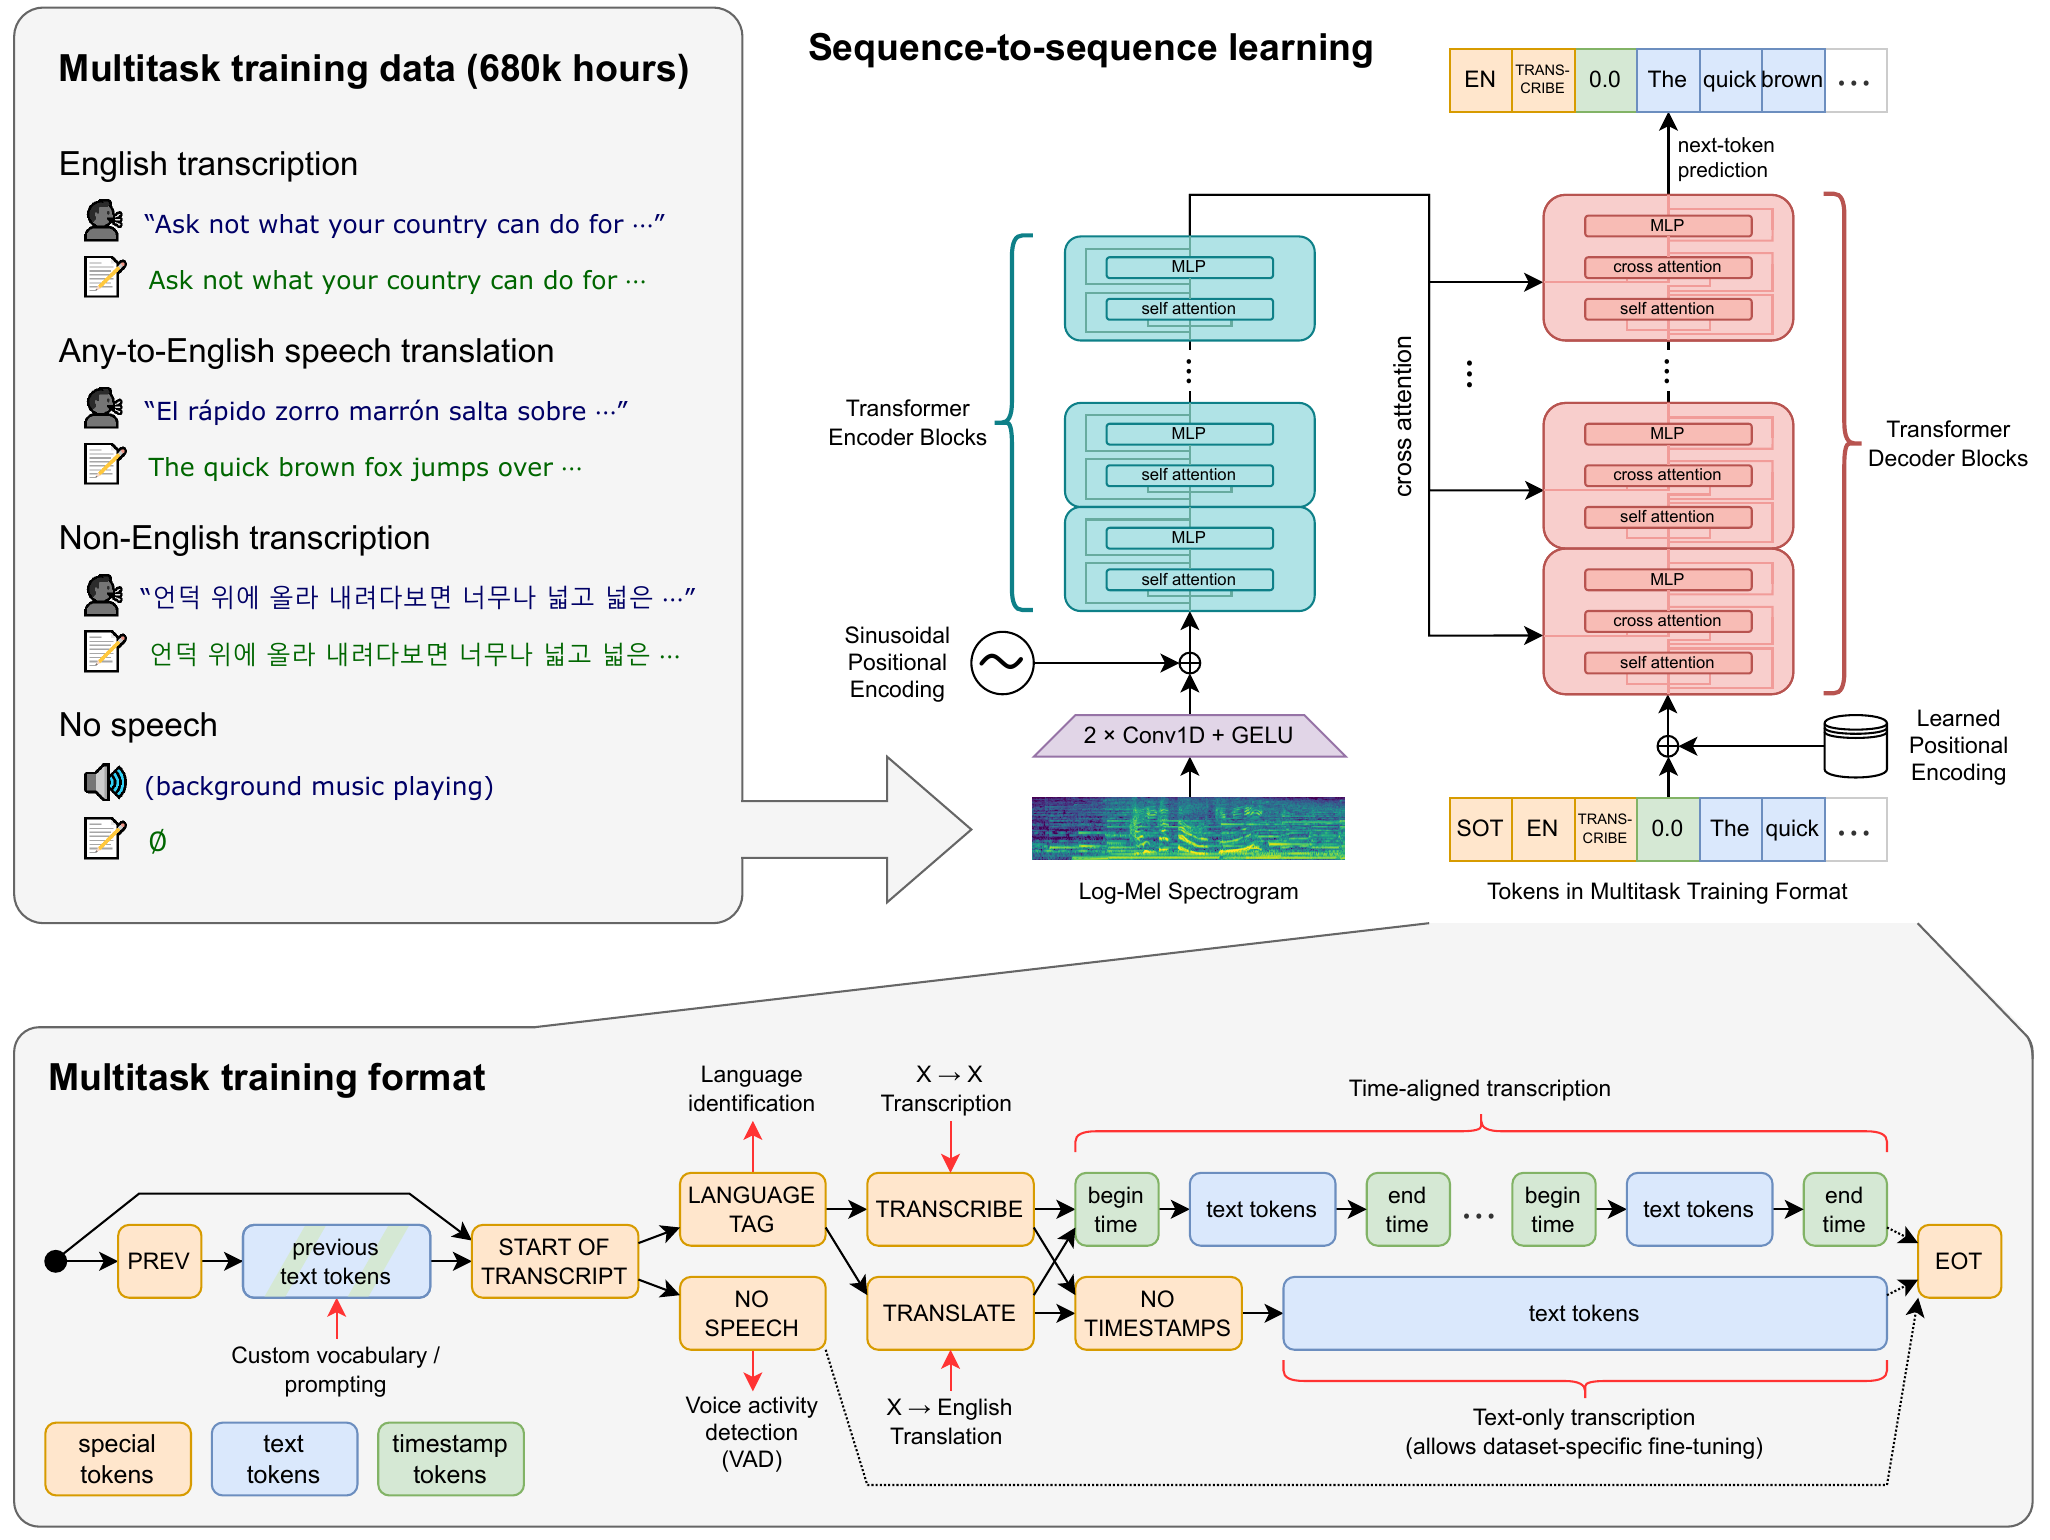
\includegraphics[width=\linewidth]{whisper_paper_figure1.png}
\caption{Kiến trúc và định dạng huấn luyện đa tác vụ của Whisper. Nguồn: trích Hình 1, Radford và cộng sự~\hyperref[ref:whisper]{[6]}. Mốc 680 nghìn giờ thuộc dữ liệu huấn luyện Whisper gốc, không phải dữ liệu huấn luyện của dự án.}
\label{fig:phowhisper-inference}
\end{figure}

\paragraph{Thu âm và chuẩn hóa tín hiệu đầu vào.}
Module \code{audio_capture.py} thu âm một kênh ở định dạng PCM int16 theo từng khối khoảng 100~ms. Tần số lấy mẫu ưu tiên là 16~kHz. Nếu microphone không hỗ trợ tần số này, chương trình thu theo tần số phù hợp với thiết bị rồi lấy mẫu lại về 16~kHz, bảo đảm tín hiệu đầu vào thống nhất với yêu cầu của mô hình.

Với mỗi khối âm thanh, chương trình trừ giá trị trung bình để giảm thành phần lệch một chiều (DC), sau đó áp dụng hệ số khuếch đại mặc định 1,8 lần. Hệ số này được giảm khi cần để biên độ đầu ra không vượt 30000 trên thang int16. Trước khi suy luận, dữ liệu được chuyển sang float32 và chia cho 32768. Các bước trên chuẩn hóa tín hiệu đầu vào; chất lượng nhận dạng vẫn phụ thuộc vào bản thu, đặc biệt khi có tiếng ồn hoặc tín hiệu bị cắt đỉnh.

\paragraph{Phát hiện tiếng nói và xác định ranh giới câu.}
Luồng âm thanh liên tục cần được chia thành các đoạn có tiếng nói trước khi đưa vào mô hình. Hệ thống sử dụng WebRTC VAD để xử lý từng khung 20~ms và bắt đầu ghi câu khi có ít nhất ba khung chứa tiếng nói trong cửa sổ năm khung gần nhất. Bộ đệm giữ khoảng 0,30~s âm thanh trước thời điểm kích hoạt nhằm hạn chế mất âm đầu. Khung 20~ms được dùng cho phát hiện tiếng nói, còn cửa sổ 25~ms nêu trên được dùng cho trích xuất đặc trưng phổ.

Câu được kết thúc sau khoảng 0,60~s không có tiếng nói. Đoạn có quá ít khung tiếng nói bị bỏ; câu dài khoảng 8~s trở lên bị từ chối thay vì lấy một phần câu để điều khiển. Ngoài bước VAD bên ngoài, lời gọi nhận dạng bật \code{vad_filter=True}, sử dụng bộ lọc Silero VAD được tích hợp trong \code{faster-whisper} để lọc thêm phần không có tiếng nói trước giải mã~\hyperref[ref:fasterwhisper]{[3]}. Hai bước có vai trò khác nhau: bước ngoài chia luồng microphone thành câu, bước trong xử lý đoạn âm thanh đã được chuyển cho thư viện. Các ngưỡng hiện tại phục vụ câu điều hướng ngắn, chưa tối ưu cho mọi cách nói chậm hoặc câu nhiều hành động.

\paragraph{Tổ chức xử lý và cấu hình giải mã.}
Node ROS \code{speech_node} quản lý một worker bằng cơ chế multiprocessing. Trong worker, luồng thu/VAD và luồng giải mã được tách riêng để việc suy luận không chặn đọc microphone hoặc callback ROS. Ngoài câu đang giải mã, hàng đợi chỉ giữ tối đa một câu chờ để hạn chế tích lũy yêu cầu cũ. Nếu mất mẫu hoặc hàng đợi đầy, hệ thống thông báo lỗi; khi robot đang điều hướng, lỗi âm thanh tạo yêu cầu hủy tuyến theo cơ chế giám sát đã cài đặt.

Các tham số suy luận chính được trình bày trong Bảng~\ref{tab:asr-settings}. Thuật toán beam search duy trì nhiều giả thuyết chuỗi token tại mỗi bước để tìm kết quả có điểm số phù hợp. Giá trị \code{beam_size=5} được lựa chọn nhằm cân bằng phạm vi tìm kiếm và thời gian xử lý; hiệu quả nhận dạng còn phụ thuộc vào tín hiệu đầu vào và mô hình.

\begin{table}[H]
\centering\small
\renewcommand{\arraystretch}{1.15}
\begin{tabularx}{\linewidth}{@{}L{4.2cm}L{2.6cm}Y@{}}
\toprule
\textbf{Tham số} & \textbf{Giá trị} & \textbf{Ý nghĩa trong dự án} \\
\midrule
\code{language} & \code{vi} & Chỉ định tiếng Việt, không cần tự phát hiện ngôn ngữ cho mỗi câu. \\
\code{task} & \code{transcribe} & Chép lại lời nói, không dịch câu sang tiếng Anh. \\
\code{beam_size} & 5 & Giữ nhiều giả thuyết khi tìm chuỗi token. \\
\code{temperature} & 0 & Không sử dụng lấy mẫu ngẫu nhiên ở bước giải mã này. \\
\code{condition_on_previous_text} & \code{False} & Không dùng văn bản đoạn trước làm ngữ cảnh giải mã đoạn tiếp theo. \\
\code{vad_filter} & \code{True} & Lọc thêm phần không có tiếng nói trong đoạn âm thanh. \\
\code{device}, \code{compute_type} & CPU, int8 & Suy luận trên CPU với trọng số đã lượng tử hóa. \\
\code{cpu_threads} & 2 & Giới hạn luồng tính toán để chia sẻ tài nguyên với mô phỏng. \\
\code{use_hotwords} & \code{False} & Mặc định không gợi ý sẵn tên phòng hoặc câu điều khiển. \\
\bottomrule
\end{tabularx}
\caption{Cấu hình nhận dạng giọng nói đang sử dụng trong mã nguồn.}
\label{tab:asr-settings}
\end{table}

\paragraph{Triển khai nhận dạng ngoại tuyến và lượng tử hóa int8.}
File \code{voice_model.py} tải trọng số mô hình và chuyển sang định dạng CTranslate2 trước lần sử dụng đầu tiên. Lượng tử hóa int8 biểu diễn các trọng số được hỗ trợ bằng số nguyên 8 bit kèm hệ số quy đổi, giúp giảm dung lượng lưu trữ và có thể cải thiện tốc độ suy luận trên phần cứng phù hợp. Kiểu dữ liệu của các phép toán còn lại phụ thuộc vào bộ thực thi~\hyperref[ref:quantization]{[7]}.

Mô hình được thực thi bằng \code{faster-whisper} trên CPU với hai luồng để chia sẻ tài nguyên với Gazebo, RViz và Nav2. Sau khi chuẩn bị trọng số, node nạp mô hình từ cache với \code{local_files_only=True}, cho phép nhận dạng tại máy mà không gửi âm thanh tới dịch vụ mạng. Quá trình chuyển định dạng và lượng tử hóa sử dụng trọng số có sẵn. Ảnh hưởng của int8 tới độ chính xác và tốc độ chưa được đo riêng trong bài thực hành.

\paragraph{Kiểm tra kết quả và chuyển sang yêu cầu điều hướng.}
Sau khi giải mã, chương trình ghép văn bản của các đoạn (segment) thành câu hoàn chỉnh. Kết quả được chuyển tiếp khi không rỗng và mỗi segment có \code{avg_logprob} không nhỏ hơn $-1{,}0$, đồng thời \code{no_speech_prob} nhỏ hơn $0{,}7$. Tham số thứ nhất là điểm log-xác suất trung bình của kết quả giải mã; tham số thứ hai thể hiện đánh giá của mô hình về khả năng không có tiếng nói. Hai ngưỡng này được dùng để lọc sơ bộ kết quả nhận dạng, chưa đủ để bảo đảm câu lệnh có nội dung chính xác.

Câu nhận dạng được gửi dưới dạng JSON trên topic \code{/voice_navigation/speech}, gồm văn bản, cờ hoàn chỉnh và dấu thời gian thu âm. Kết quả có tuổi quá 10~s bị loại bỏ. Node điều hướng cũng bỏ qua câu bắt đầu thu trước yêu cầu dừng nếu kết quả giải mã được trả về sau yêu cầu đó. Giao diện hiển thị nguyên văn kết quả nhận dạng để người dùng kiểm tra.

Sau bước ASR, module \code{commands.py} kiểm tra mẫu câu và tra cứu tên khu vực theo các ví dụ trong Bảng~\ref{tab:commands}. Toàn bộ điểm đến phải được xác định hợp lệ trước khi hệ thống gửi mục tiêu đầu tiên. Bộ phân tích hiện sử dụng quy tắc cho các mẫu câu điều hướng đã hỗ trợ; khả năng hiểu câu dài với nhiều loại hành động được đề xuất trong phần hướng phát triển.

\begin{table}[H]
\centering\small
\renewcommand{\arraystretch}{1.15}
\begin{tabularx}{\linewidth}{@{}L{7.5cm}Y@{}}
\toprule
\textbf{Ví dụ câu lệnh} & \textbf{Kết quả phân tích} \\
\midrule
Đi vào phòng ngủ. & Tuyến $[A]$. \\
Di chuyển vào phòng sinh hoạt. & Tuyến $[B]$. \\
Đi ra hành lang. & Tuyến $[C]$. \\
Đi từ nhà bếp ra phòng khách. & Tuyến $[E,D]$. \\
Đi từ phòng A qua hành lang C rồi đến phòng B. & Tuyến $[A,C,B]$. \\
Đi vào phòng vệ sinh. & Từ chối: tên không có trong YAML. \\
Dừng lại / Dừng robot / Hủy lệnh. & Yêu cầu hủy hành trình hiện tại. \\
\bottomrule
\end{tabularx}
\caption{Ánh xạ câu lệnh thành tuyến hoặc yêu cầu hủy. Bảng mô tả quy tắc phân tích văn bản.}
\label{tab:commands}
\end{table}

\FloatBarrier
\subsection{Chuyển tọa độ pixel sang hệ tọa độ bản đồ}

Ảnh có gốc ở góc trên trái, còn bản đồ ROS sử dụng gốc và hướng trong \code{map.yaml}. Gọi $u,v$ là chỉ số cột và hàng pixel, $H$ là số hàng, $r$ là độ phân giải. Tọa độ tâm ô trong hệ cục bộ được tính bằng:
\begin{equation}
 x_\ell=(u+0{,}5)r,\qquad y_\ell=(H-v-0{,}5)r.
\end{equation}
Với origin $(o_x,o_y,\theta)$, phép đổi sang frame \code{map} là:
\begin{align}
 x &= o_x+\cos\theta\,x_\ell-\sin\theta\,y_\ell,\\
 y &= o_y+\sin\theta\,x_\ell+\cos\theta\,y_\ell.
\end{align}
Bản đồ hiện có origin $(-9{,}32;-5{,}52;0)$. Thành phần $+0{,}5$ giúp lấy tâm ô thay vì góc ô; phép đảo hàng xử lý chiều trục tung của ảnh. \code{map_tools.py} cũng có phép đổi ngược để đưa polygon và goal từ mét về pixel. Khi gửi goal, góc hướng $\psi$ được đổi thành quaternion phẳng với $q_z=\sin(\psi/2)$ và $q_w=\cos(\psi/2)$.

\subsection{Thực hiện nhiều điểm đến và xử lý lệnh dừng}

\paragraph{Định vị, lập đường và điều khiển.}
Sau khi xác định được điểm đích, robot cần biết vị trí hiện tại và tính cách di chuyển phù hợp. Hệ thống sử dụng các thành phần của Nav2 với vai trò sau:
\begin{itemize}
\item \textbf{AMCL:} ước lượng tư thế robot trên bản đồ đã lưu bằng bộ lọc hạt, kết hợp thông tin chuyển động từ odometry với phép đo LiDAR. AMCL cung cấp phép biến đổi giữa hệ \code{map} và \code{odom}, từ đó liên kết vị trí robot với hệ tọa độ mục tiêu~\hyperref[ref:localization]{[8]}.
\item \textbf{NavFn:} tính đường toàn cục từ vị trí hiện tại tới đích trên global costmap. Trong \code{nav2.yaml}, tham số \code{use_astar=false} lựa chọn chế độ mở rộng Dijkstra~\hyperref[ref:navfn]{[9]}.
\item \textbf{DWB:} lấy mẫu các vận tốc ứng viên, mô phỏng quỹ đạo ngắn hạn và chấm điểm theo các tiêu chí như khoảng cách tới đường kế hoạch, tới đích và mức độ gần vật cản. Bộ điều khiển lựa chọn vận tốc phù hợp trong giới hạn cấu hình để robot bám đường~\hyperref[ref:dwb]{[10]}.
\item \textbf{Costmap:} kết hợp thông tin bản đồ tĩnh và cảm biến thành lưới chi phí phục vụ planner và controller. Lớp inflation tăng chi phí quanh vật cản nhằm ưu tiên đường có khoảng cách phù hợp với chúng~\hyperref[ref:inflation]{[11]}.
\end{itemize}

Trong cấu hình hiện tại, bán kính robot là 0,175~m và \code{inflation_radius} là 0,45~m. Bán kính inflation xác định phạm vi lan truyền chi phí, không có nghĩa toàn bộ phạm vi đó đều bị cấm đi. Khoảng hở $m$ trong bước chọn đích và các tham số costmap có vai trò khác nhau: bước chọn đích lọc ứng viên trên bản đồ lưu sẵn, còn costmap phục vụ lập đường và điều khiển khi chạy. Vì vậy, một điểm đích hợp lệ trên ảnh vẫn có thể không tới được khi xuất hiện vật cản mới hoặc định vị sai.

\paragraph{Thực hiện tuần tự các mục tiêu.}


Node điều hướng sử dụng action \code{NavigateToPose} của Nav2, gồm goal vị trí và phản hồi kết quả~\hyperref[ref:nav2]{[4]}. Với tuyến $R=[r_0,r_1,\ldots,r_{n-1}]$, node lưu chỉ số chặng $i$, gửi goal của $r_i$ và chỉ chuyển sang $i+1$ khi nhận \code{STATUS_SUCCEEDED}. Vì vậy, câu ``đi từ A đến B'' vẫn tạo goal A trước B ngay cả khi robot đang ở nơi khác. Hiện chưa suy luận từ pose để tự bỏ qua chặng đầu khi robot đã ở trong vùng A.

Ngưỡng kiểm tra goal đang đặt 0,25~m cho vị trí và 0,25~rad cho hướng; đây là tham số cấu hình, không phải sai số thực nghiệm đã đo. Nếu một chặng thất bại, bị từ chối hoặc quá thời gian 180~s, node không chuyển sang điểm sau.

\begin{figure}[H]
\centering
\resizebox{0.96\linewidth}{!}{%
\begin{tikzpicture}[
    statebox/.style={draw=blue!65!black,rounded corners=4pt,fill=blue!5,
        align=center,text width=3.2cm,minimum height=1.7cm,inner sep=6pt,
        font=\fontsize{10.5}{12.5}\selectfont},
    transition/.style={-{Stealth[length=2.2mm]},thick,draw=blue!65!black},
    event/.style={font=\fontsize{9}{11}\selectfont,align=center,
                  fill=white,inner sep=3pt}
]
\node[statebox] (idle) at (0,0) {\textbf{CHỜ}\\Nhận yêu cầu mới};
\node[statebox] (validate) at (6.5,0) {\textbf{KIỂM TRA}\\Mẫu câu, tên vùng, Nav2};
\node[statebox,fill=green!8,draw=green!45!black] (running) at (13,0)
    {\textbf{ĐIỀU HƯỚNG}\\Gửi goal chặng $i$};
\node[statebox,fill=yellow!12,draw=orange!80!black] (result) at (13,-4.7)
    {\textbf{KẾT QUẢ / HỦY}\\Hoàn tất, lỗi hoặc dừng};

\draw[transition] (idle.east) -- node[event,above=3pt] {Câu nói / GUI} (validate.west);
\draw[transition] (validate.east) -- node[event,above=3pt] {Hợp lệ} (running.west);

% Nhánh từ chối nằm phía dưới hai khối đầu, nhãn có chiều rộng cố định.
\draw[transition] (validate.south) -- (6.5,-2.3)
    -- node[event,below=3pt,text width=5cm]
       {Tên vùng lạ / sai mẫu câu\\hoặc Nav2 chưa sẵn sàng} (0,-2.3)
    -- (idle.south);

% Vòng lặp chỉ vòng ngoài khối đang chạy, không cắt qua khối kiểm tra.
\draw[transition] (running.north) -- (13,2.2)
    -- node[event,above=3pt,text width=4.2cm]
       {Chặng thành công, còn điểm\\Tăng $i$, gửi goal kế tiếp} (16.5,2.2)
    -- (16.5,0) -- (running.east);

\draw[transition] (running.south)
    -- node[event,right=4pt,text width=2.8cm]
       {Hết tuyến / lỗi\\hoặc yêu cầu dừng} (result.north);

% Đường về trạng thái chờ đi vòng bên trái, tách khỏi nhánh từ chối.
\draw[transition] (result.west)
    -- node[event,above=3pt] {Chờ yêu cầu mới} (-3.1,-4.7)
    -- (-3.1,0) -- (idle.west);
\node[event,anchor=north,text width=16cm] at (6.5,-6.7)
    {Không nhận tuyến mới khi robot đang bận.\\
     Lệnh dừng được xét trước điều kiện bận; yêu cầu hủy phải chờ phản hồi Nav2.};
\end{tikzpicture}%
}
\caption{Quy trình kiểm tra và thực hiện tuyến nhiều điểm đến.}
\label{fig:navigation-states}
\end{figure}

Lệnh dừng được ưu tiên xử lý ngay cả khi robot đang thực hiện hành trình, thông qua hàm \code{cancel_goal_async()}. Nếu mục tiêu chưa được Nav2 chấp nhận, node ghi nhận cờ hủy và gửi yêu cầu hủy ngay sau khi nhận phản hồi chấp nhận. Giao diện duy trì trạng thái chờ cho tới khi có phản hồi từ Nav2. Sau khi hủy hành trình, người dùng cần gửi yêu cầu mới để tiếp tục điều hướng.

Cơ chế kiểm tra dấu thời gian giúp hạn chế thực hiện lại câu lệnh cũ sau khi dừng. Khi phát hiện lỗi âm thanh hoặc hàng đợi giải mã đầy trong quá trình điều hướng, hệ thống tạo yêu cầu hủy tuyến. Nút \textbf{DỪNG ROBOT} trên giao diện gửi yêu cầu hủy trực tiếp, còn lệnh dừng bằng giọng nói cần qua bước nhận dạng. Cả hai cách đều sử dụng cơ chế hủy mục tiêu của Nav2, không tác động trực tiếp tới nguồn động cơ.

\Needspace{4\baselineskip}
\section{Hình ảnh kết quả thực nghiệm}

\subsection{Nhận dạng câu lệnh và hiển thị bản đồ}

Các ảnh thực nghiệm trong thư mục \code{ketqua/} minh họa kết quả nhận dạng câu lệnh, bản đồ phân vùng A--E, tuyến điều hướng và trạng thái kết nối Nav2. Ba trường hợp dưới đây tương ứng với yêu cầu tới phòng ngủ, phòng sinh hoạt và hành lang. Phần nhận xét tập trung vào thông tin hiển thị tại thời điểm chụp; các chỉ số định lượng được nêu trong phần hạn chế.

\begin{figure}[H]
\centering
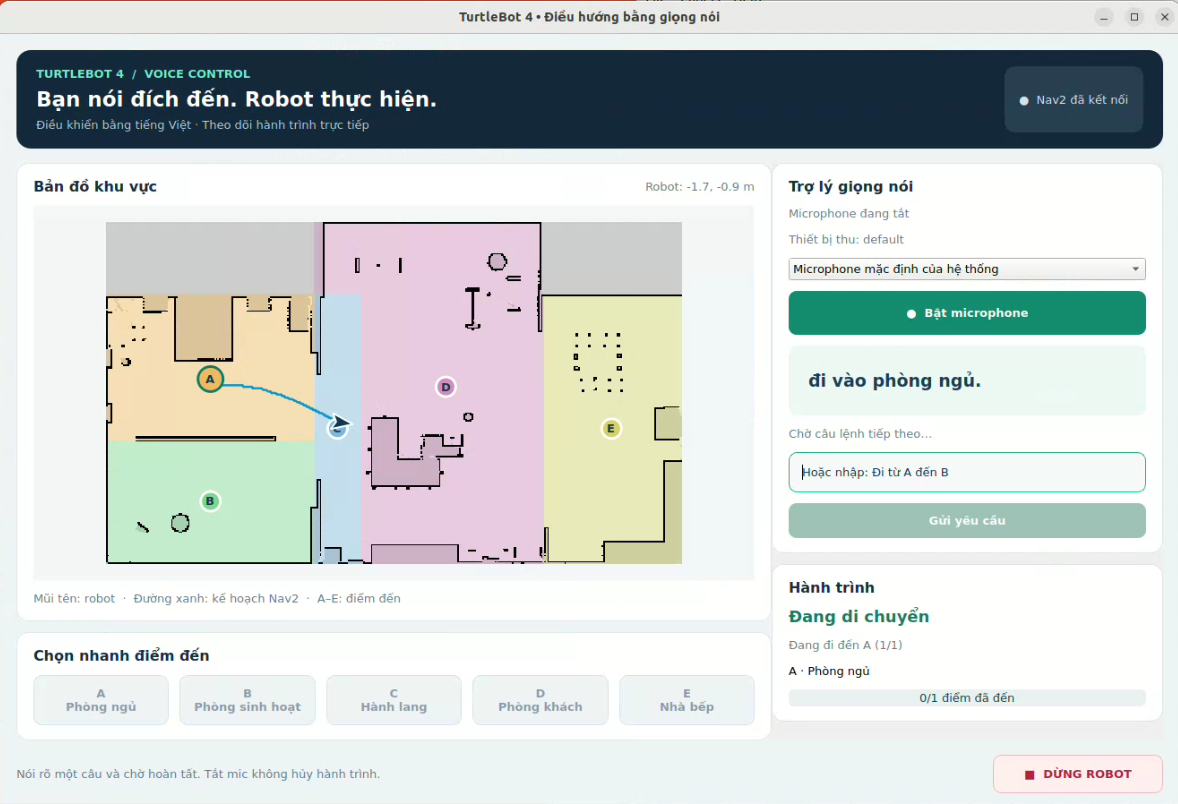
\includegraphics[width=0.94\linewidth]{phongngu.png}
\caption{Câu ``đi vào phòng ngủ'' được gắn với đích A; GUI hiển thị đường Nav2 và trạng thái đang di chuyển.}
\label{fig:bedroom}
\end{figure}

Trong Hình~\ref{fig:bedroom}, câu ``đi vào phòng ngủ'' được ánh xạ tới đích A. Giao diện đánh dấu đích trên bản đồ, hiển thị đường Nav2 màu xanh và trạng thái ``Đang đi đến A (1/1)'', với tiến độ 0/1. Tại thời điểm này, robot đang thực hiện chặng tới phòng ngủ. Microphone đã tắt nhưng hành trình vẫn tiếp tục, thể hiện hai thao tác tắt thu âm và hủy mục tiêu được xử lý độc lập.

\begin{figure}[H]
\centering
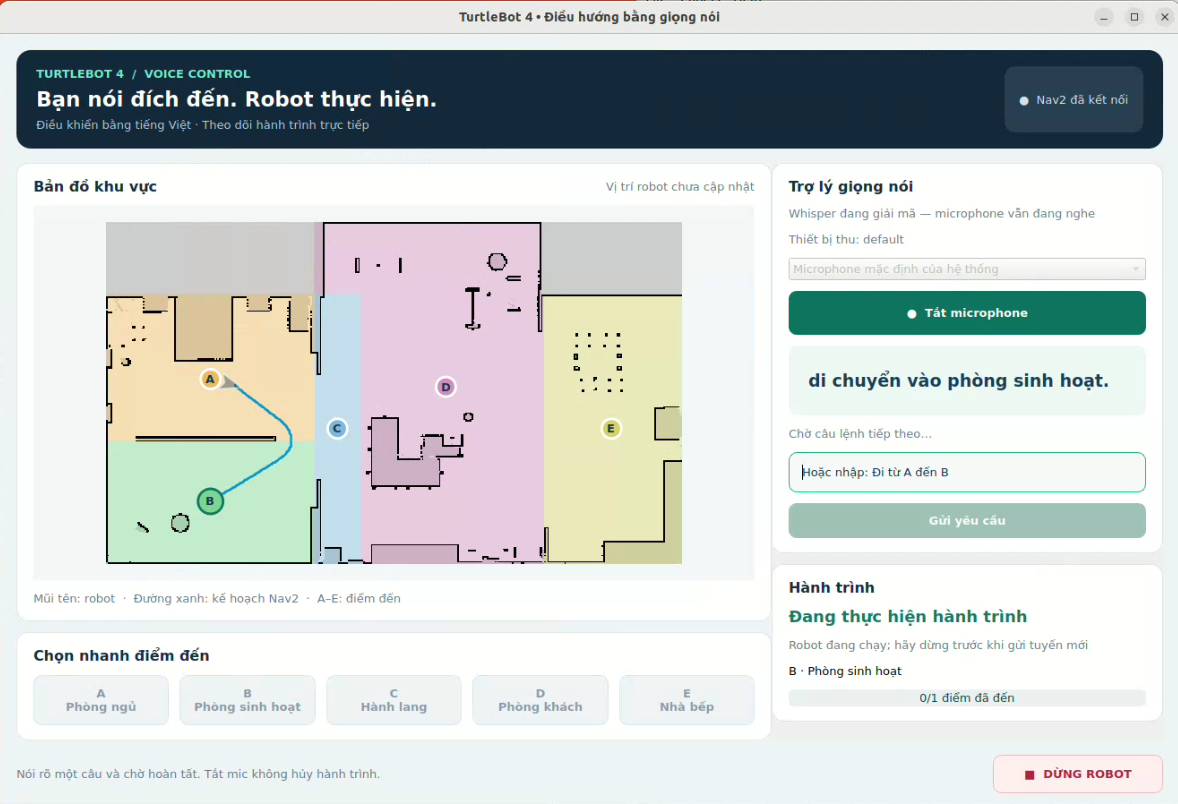
\includegraphics[width=0.94\linewidth]{phongsh.png}
\caption{Câu ``di chuyển vào phòng sinh hoạt'' tương ứng đích B; hệ thống đang bận với hành trình hiện tại.}
\label{fig:activity-room}
\end{figure}

Hình~\ref{fig:activity-room} hiển thị câu ``di chuyển vào phòng sinh hoạt'' và tuyến tới đích B. Thông báo ``Robot đang chạy; hãy dừng trước khi gửi tuyến mới'' cho thấy hệ thống từ chối nhận thêm tuyến khi đang thực hiện hành trình. Giao diện đồng thời cảnh báo dữ liệu vị trí chưa được cập nhật; đây là vấn đề cần kiểm tra thêm ở khâu đồng bộ với AMCL.

\begin{figure}[H]
\centering
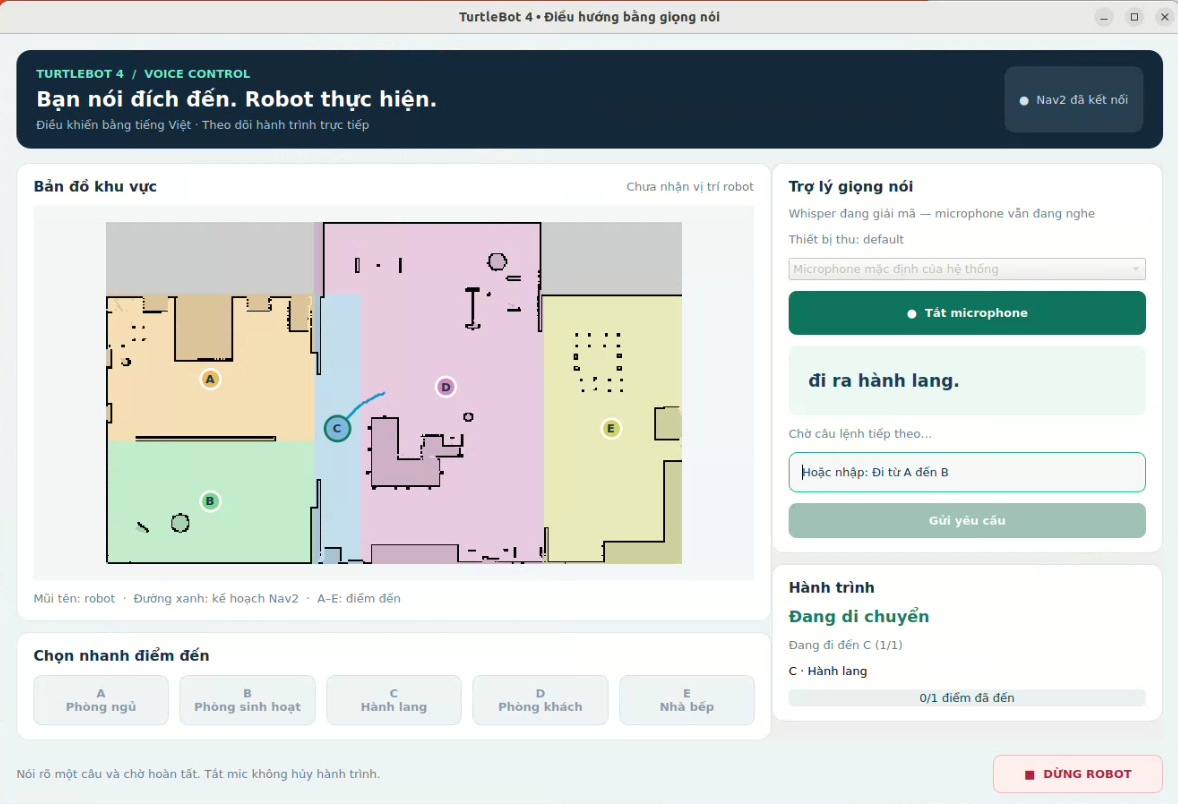
\includegraphics[width=0.94\linewidth]{hanhlang.png}
\caption{Câu ``đi ra hành lang'' được phân tích thành đích C và chuyển sang điều hướng.}
\label{fig:corridor}
\end{figure}

Hình~\ref{fig:corridor} minh họa kết quả xử lý mẫu câu ``đi ra hành lang''. Hệ thống xác định đích C, hiển thị đường kế hoạch của chặng hiện tại và trạng thái ``Đang đi đến C (1/1)''. Kết quả cho thấy bộ phân tích hỗ trợ cách diễn đạt ``đi ra'' bên cạnh ``đi đến''. Tuy nhiên, giao diện chưa nhận được vị trí robot tại thời điểm chụp.

\subsection{Kết quả điều hướng và xử lý tình huống}

\paragraph{Điều hướng nhiều điểm theo thứ tự.}
Câu ``đi từ phòng ngủ qua hành lang rồi vào phòng sinh hoạt'' được phân tích thành tuyến $[A,C,B]$. Trong Hình~\ref{fig:multi-goal}, giao diện hiển thị đúng thứ tự ba khu vực và thông báo ``Đã đến đủ các khu vực theo thứ tự'', với tiến độ 3/3. Kết quả này ghi nhận trạng thái hoàn tất cả ba chặng do node điều hướng cung cấp. Quỹ đạo thực tế của robot có thể được đối chiếu thêm qua video và dữ liệu vị trí.

\begin{figure}[!htbp]
\centering
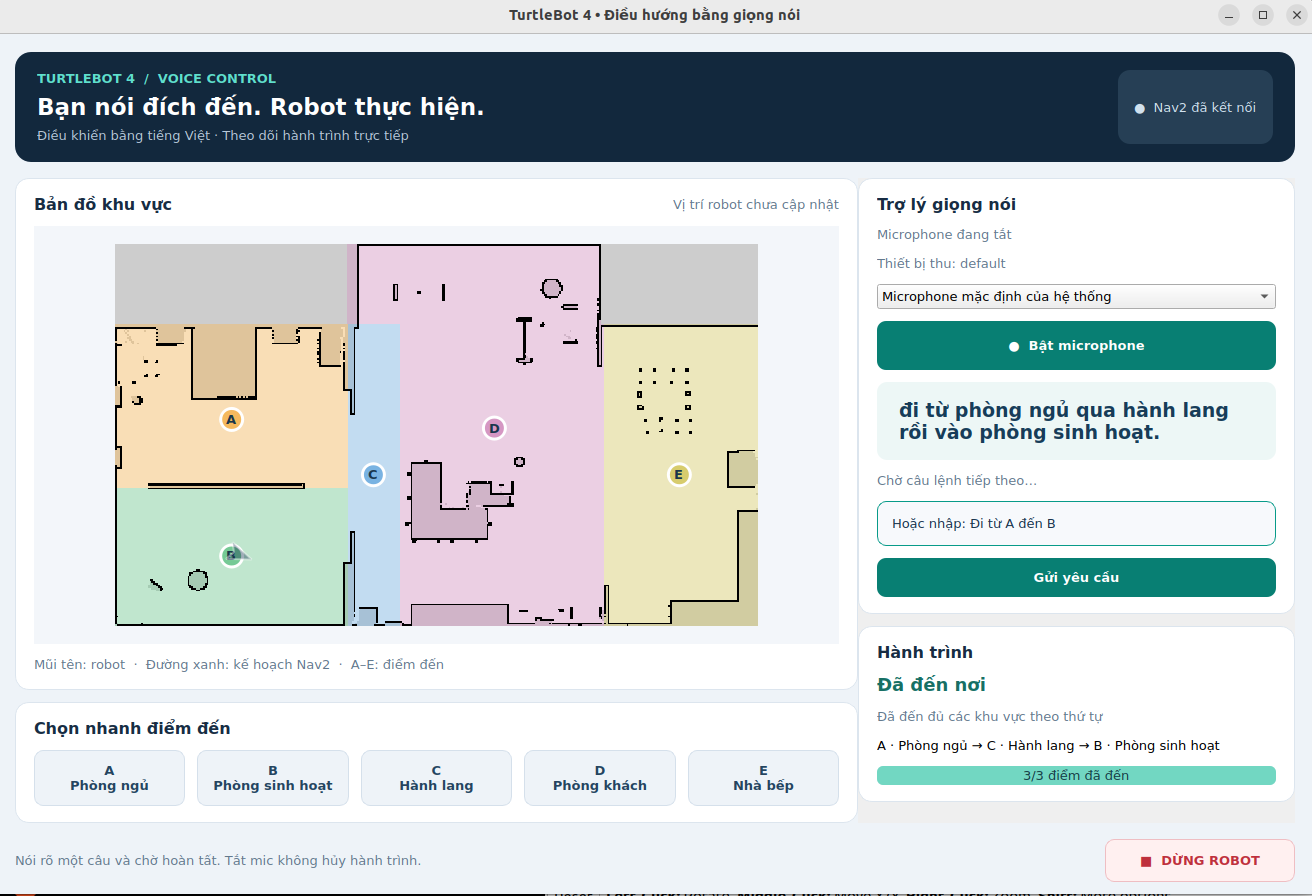
\includegraphics[width=0.94\linewidth]{nhieudiemden.png}
\caption{Hoàn tất tuyến A (phòng ngủ) $\rightarrow$ C (hành lang) $\rightarrow$ B (phòng sinh hoạt), tiến độ 3/3 trên giao diện.}
\label{fig:multi-goal}
\end{figure}

Đối với chức năng nhiều điểm đến, giao diện hiển thị danh sách các khu vực theo thứ tự và đường Nav2 của chặng đang thực hiện. Chức năng tính trước và hiển thị đường đi liên tục qua toàn bộ tuyến A--C--B chưa được triển khai.

\paragraph{Khu vực không tồn tại.}
Trong Hình~\ref{fig:unknown-region}, câu ``đi vào phòng vệ sinh'' bị từ chối do tên khu vực không có trong dữ liệu A--E. Giao diện hiển thị thông báo ``Khu vực không tồn tại'' và liệt kê các ID hợp lệ. Việc kiểm tra được thực hiện trước khi gửi mục tiêu cho Nav2. Với câu lệnh nhiều chặng, toàn bộ tuyến cũng bị từ chối nếu có một tên khu vực không hợp lệ.

\begin{figure}[!htbp]
\centering
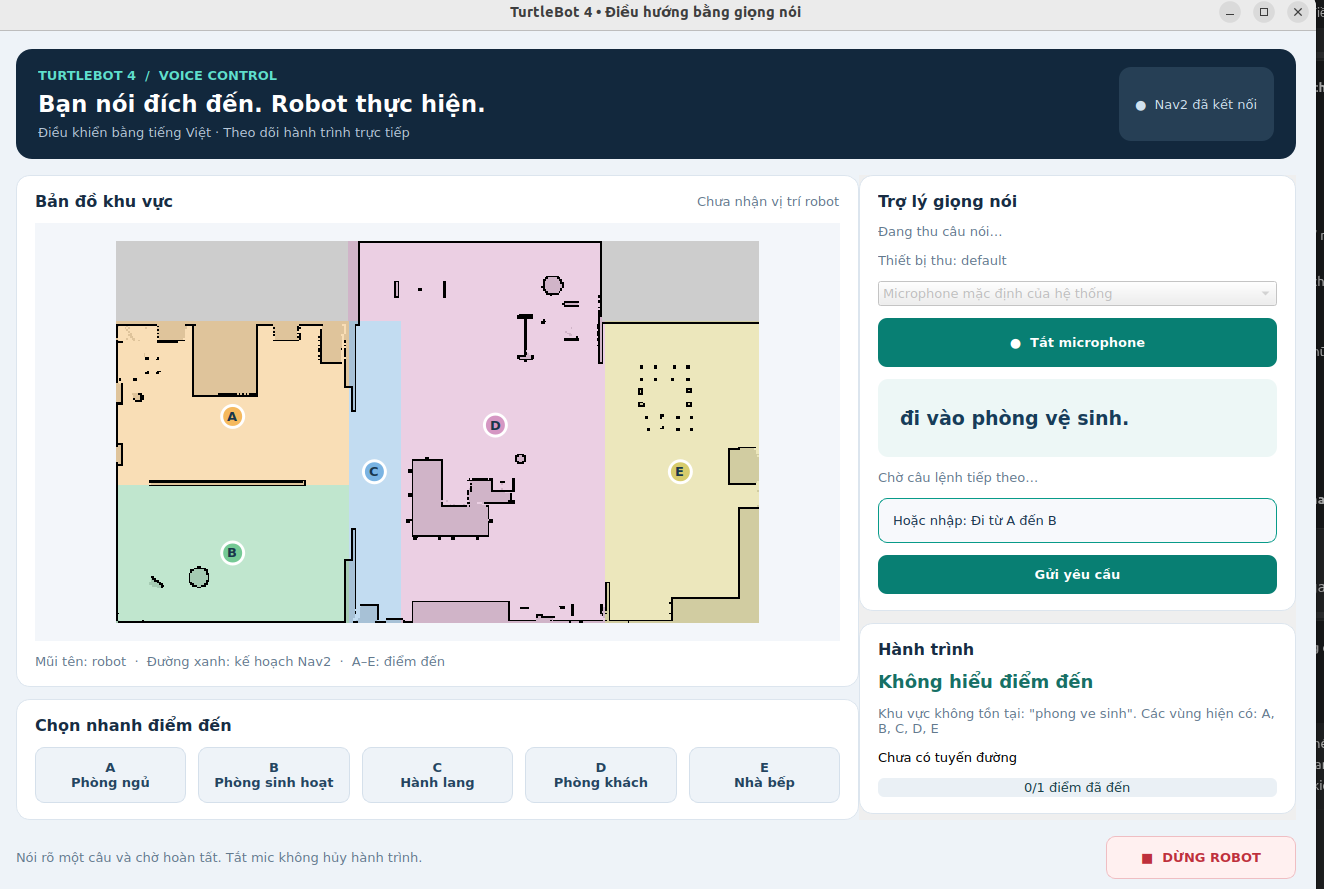
\includegraphics[width=0.94\linewidth]{falled.png}
\caption{Từ chối yêu cầu tới phòng vệ sinh vì khu vực này không có trong dữ liệu ngữ nghĩa.}
\label{fig:unknown-region}
\end{figure}

\paragraph{Nhận xét từ các ảnh thực nghiệm.}
Các ảnh thực nghiệm minh họa ba cách gọi đích đơn, một tuyến nhiều điểm và một trường hợp khu vực không tồn tại. Hệ thống đã hiển thị kết quả ánh xạ và phản hồi tương ứng cho từng tình huống. Bên cạnh đó, cảnh báo dữ liệu vị trí trên một số ảnh cho thấy cần kiểm tra thêm việc đồng bộ giao diện với AMCL. Trạng thái ``Nav2 đã kết nối'' phản ánh khả năng truy cập action server; tình trạng định vị và cảm biến cần được theo dõi riêng.

\FloatBarrier
\Needspace{4\baselineskip}
\section{Đánh giá kết quả và hướng phát triển}

\subsection{Kết quả đạt được}

Qua bài thực hành, em đã xây dựng được quy trình kết hợp bản đồ ngữ nghĩa, nhận dạng tiếng Việt và điều hướng bằng Nav2. Bản đồ được chia thành năm vùng có tên, tên gọi thay thế và điểm đích trên ô trống, đáp ứng yêu cầu tối thiểu ba khu vực. Dữ liệu trong \code{map.yaml} được sử dụng để thống nhất tọa độ giữa ảnh phân vùng, giao diện và mục tiêu điều hướng.

Các ảnh thực nghiệm ghi nhận văn bản của ba câu ``đi vào phòng ngủ'', ``di chuyển vào phòng sinh hoạt'' và ``đi ra hành lang'', cùng trạng thái điều hướng tương ứng. Tuyến A--C--B có trạng thái hoàn tất 3/3; yêu cầu tới phòng vệ sinh bị từ chối vì tên không tồn tại. Các kết quả này minh họa khả năng nhận lệnh một điểm, nhiều điểm và kiểm tra dữ liệu đầu vào. Nav2 đảm nhiệm việc lập đường và tránh vật cản, thay cho phát lệnh tiến/quay cố định từ node giọng nói.

Giao diện đồ họa hỗ trợ theo dõi câu nhận dạng, tên đích, thứ tự các khu vực và đường đi của chặng hiện tại. Người dùng có thể gửi yêu cầu bằng giọng nói, nhập văn bản, chọn khu vực hoặc hủy hành trình bằng nút dừng. Để giảm tải hiển thị, môi trường mô phỏng được giảm số nguồn sáng từ tám xuống một và điều chỉnh tần số gửi trạng thái hiển thị xuống 20~Hz, trong khi giữ nguyên hình học, va chạm và tần số cảm biến. Hiệu quả giảm tải chưa được đánh giá bằng số đo tốc độ khung hình hoặc hệ số thời gian thực.

\subsection{Phương pháp đánh giá đề xuất}

Để đánh giá đầy đủ hơn các chức năng đã minh họa, cần kiểm tra riêng từng khâu và toàn bộ quá trình từ giọng nói tới chuyển động. Phần này xác định tiêu chí cho các lần thử bổ sung; báo cáo hiện chưa có bộ dữ liệu và số lần lặp đủ để tính các chỉ số dưới đây.

\paragraph{Thiết kế các tình huống thử.}
Bộ câu nên bao gồm yêu cầu một điểm, nhiều điểm, tên khu vực không tồn tại và lệnh dừng khi robot đang chạy. Mỗi câu được lặp lại trong cùng điều kiện microphone, khoảng cách thu và cấu hình mô hình; khi khảo sát tiếng ồn cần tách thành nhóm riêng. Ví dụ, có thể bắt đầu với năm lần lặp cho mỗi câu để quan sát lỗi, sau đó tăng số mẫu trước khi kết luận về độ ổn định. Với điều hướng, cần ghi vị trí xuất phát, trạng thái dock, thời điểm gửi mục tiêu và kết quả từng chặng. Các lần gửi lại sau lỗi được ghi thành lượt thử mới.

\paragraph{Đánh giá văn bản và tuyến điểm đến.}
Tỷ lệ lỗi từ (Word Error Rate -- WER) được tính bằng~\hyperref[ref:wer]{[12]}:
\begin{equation}
 \mathrm{WER}=\frac{S+D+I}{N_{\mathrm{ref}}}\times100\%,
\end{equation}
trong đó $S$, $D$, $I$ lần lượt là số đơn vị bị thay thế, bị xóa và được chèn thêm sau khi căn chỉnh văn bản; $N_{\mathrm{ref}}$ là số đơn vị trong bản chép lời đối chiếu. Khi thực hiện cần thống nhất cách chuẩn hóa Unicode, chữ hoa/thường và dấu câu, đồng thời giữ dấu tiếng Việt. Nếu tách đơn vị bằng khoảng trắng, kết quả đối với tiếng Việt được hiểu theo đơn vị cách trắng, không hoàn toàn tương ứng với từ vựng đã được tách từ.

WER phản ánh sai khác văn bản nhưng chưa thể hiện đầy đủ mức độ đúng của yêu cầu điều hướng. Ví dụ, hai cách nói ``đi đến phòng ngủ'' và ``đi tới phòng ngủ'' khác văn bản nhưng cùng chỉ đích A; ngược lại, sai một tên phòng có thể thay đổi toàn bộ mục tiêu. Vì vậy, cần đánh giá thêm tỷ lệ xác định chính xác cả danh sách điểm đến và thứ tự của chúng.

\begin{table}[!htbp]
\centering\small
\renewcommand{\arraystretch}{1.15}
\begin{tabularx}{\linewidth}{@{}L{3.7cm}Y@{}}
\toprule
\textbf{Tiêu chí} & \textbf{Cách xác định trong các lần thử bổ sung} \\
\midrule
Đúng tuyến từ giọng nói & Số lượt có danh sách ID và thứ tự đúng chia cho tổng lượt nói câu điều hướng hợp lệ. Kết quả không nhận được văn bản hoặc bị từ chối cũng được tính là lượt chưa đúng. \\
Hoàn thành đầu cuối & Số lượt nhận đúng tuyến và hoàn tất mọi chặng theo thứ tự chia cho tổng lượt nói câu điều hướng hợp lệ. \\
Thành công điều hướng & Số tuyến hoàn tất chia cho số tuyến hợp lệ đã được Nav2 chấp nhận. Khi đo riêng khâu này, nhập văn bản để giảm ảnh hưởng lỗi ASR. \\
Từ chối vùng lạ & Số lượt từ chối đúng và không gửi goal chia cho tổng lượt thử có tên vùng không tồn tại. \\
Thời gian phản hồi & Đo riêng thời gian từ lúc kết thúc lời nói tới lúc có văn bản và từ lúc có văn bản tới lúc goal được chấp nhận; báo cáo số lượt, giá trị trung bình và độ phân tán. \\
\bottomrule
\end{tabularx}
\caption{Các tiêu chí đánh giá đề xuất; chưa trình bày số liệu đo thực nghiệm.}
\label{tab:evaluation-criteria}
\end{table}

\paragraph{Kiểm tra tới đích và phản hồi dừng.}
Kết quả \code{STATUS_SUCCEEDED} của từng action cần được đối chiếu với dữ liệu vị trí và video liên tục. Sai số vị trí cuối chặng có thể tính bằng $e_p=\sqrt{(x-x_g)^2+(y-y_g)^2}$, trong đó $(x_g,y_g)$ là đích và $(x,y)$ là vị trí tại thời điểm kết thúc. Khi dùng AMCL, đây là sai số theo vị trí ước lượng; nếu cần kiểm chứng độc lập trong mô phỏng, sử dụng pose thật của Gazebo sau khi thống nhất hệ tọa độ. Với lệnh dừng, cần phân biệt thời điểm nhận câu lệnh, Nav2 xác nhận hủy và robot thực sự ngừng chuyển động. Các mốc đo độ trễ phải sử dụng cùng cơ sở thời gian, tránh trộn đồng hồ mô phỏng với đồng hồ thực.

\subsection{Hạn chế của kết quả thực nghiệm}

Phương pháp phân vùng còn phụ thuộc vào polygon khai báo thủ công, chưa tự phát hiện cửa và ranh giới phòng. Điểm đích được kiểm tra trên bản đồ SLAM có sẵn, trong khi độ khớp giữa bản đồ và các chi tiết nội thất mô phỏng chưa được đánh giá đầy đủ. Do đó, khả năng di chuyển thực tế còn phụ thuộc vào chất lượng định vị, dữ liệu LiDAR, TF và cấu hình costmap.

Về nhận dạng giọng nói, PhoWhisper-small vẫn có thể nhận sai âm đầu hoặc tên phòng. Quá trình suy luận trên CPU phải chia sẻ tài nguyên với Gazebo, RViz và Nav2. Bài thực hành chưa xây dựng tập bản thu có văn bản đối chiếu, chưa có thống kê số lần thử, tỷ lệ nhận dạng đúng, tỷ lệ điều hướng thành công và thời gian phản hồi. Vì vậy, các kết quả hiện tại chủ yếu có ý nghĩa minh họa chức năng, chưa đủ để so sánh định lượng Whisper-small với PhoWhisper-small.

Bộ phân tích mới hỗ trợ các mẫu câu điều hướng và chuỗi điểm đến, chưa xử lý các hành động như ``đợi 5 giây'' hoặc ``quay trái''. Giới hạn thời lượng câu khoảng 8~s và tuổi kết quả 10~s cũng hạn chế việc tiếp nhận yêu cầu dài. Độ trễ của lệnh dừng bằng giọng nói chưa được đo riêng. Ngoài ra, dữ liệu AMCL trên giao diện còn xuất hiện trạng thái chậm cập nhật trong một số ảnh thực nghiệm.

\subsection{Hướng cải thiện}

Hướng cải thiện đầu tiên là xây dựng tập bản thu có văn bản đối chiếu và thực hiện các phép đo trong Bảng~\ref{tab:evaluation-criteria}. Khi so sánh các mô hình, cần sử dụng cùng bản thu và điều kiện phần cứng. Kết quả đo sẽ hỗ trợ lựa chọn mô hình và cấu hình CPU/GPU phù hợp.

Đối với bản đồ, có thể thử nghiệm morphology hoặc watershed kết hợp khoảng cách tới tường để đề xuất các vùng tự động, sau đó cho phép chỉnh sửa tên và ranh giới. Đối với điều hướng nhiều điểm, hướng mở rộng là tính trước các đoạn đường bằng Nav2 và hiển thị toàn tuyến, đồng thời cập nhật khi có thay đổi. Việc đánh giá cần bổ sung dữ liệu vị trí, \code{/plan}, kết quả action và video liên tục để kiểm tra thứ tự tới đích, sai số dừng và phản hồi khi hủy.

Để hỗ trợ câu dài gồm nhiều loại hành động, hệ thống cần có cấu trúc biểu diễn kế hoạch, cơ chế kiểm tra từng bước và khả năng hủy toàn bộ kế hoạch. Khâu thu âm cũng cần được điều chỉnh theo độ dài câu, kết hợp xử lý các yêu cầu mơ hồ trước khi thực thi. Đây là các hướng phát triển tiếp theo của dự án.

\section{Video demo và mã nguồn}

Video minh họa quá trình vận hành và mã nguồn của bài thực hành được cung cấp tại các liên kết dưới đây.

\begin{itemize}
  \item Video demo: \href{https://drive.google.com/drive/u/0/folders/1khVZZDVxWRnYRrrD_zvH0FuS1wvLYElE}{\underline{Google Drive -- Video demo Bài 7}}.
  \item GitHub repository: \href{https://github.com/vanthudat/Voice_Navi}{\underline{GitHub -- Mã nguồn Voice Navi}}.
\end{itemize}

\section*{Tài liệu tham khảo}
\addcontentsline{toc}{section}{Tài liệu tham khảo}
\begin{enumerate}[label={[\arabic*]},leftmargin=2em]
    \item \label{ref:opencv} OpenCV Documentation, \textit{Miscellaneous Image Transformations: distanceTransform}.\\
    \url{https://docs.opencv.org/4.x/d7/d1b/group__imgproc__misc.html}
    \item \label{ref:phowhisper} Thanh-Thien Le, Linh The Nguyen và Dat Quoc Nguyen, \textit{PhoWhisper: Automatic Speech Recognition for Vietnamese}, ICLR 2024 Tiny Papers.\\
    \url{https://github.com/VinAIResearch/PhoWhisper}
    \item \label{ref:fasterwhisper} SYSTRAN, \textit{Faster Whisper transcription with CTranslate2}.\\
    \url{https://github.com/SYSTRAN/faster-whisper}
    \item \label{ref:nav2} Navigation2, \textit{NavigateToPose action}, mã nguồn nhánh Humble.\\
    \url{https://github.com/ros-navigation/navigation2/blob/humble/nav2_msgs/action/NavigateToPose.action}
    \item \label{ref:tb4sim} TurtleBot 4 User Manual, \textit{TurtleBot 4 Simulator}.\\
    \url{https://turtlebot.github.io/turtlebot4-user-manual/software/turtlebot4_simulator.html}
    \item \label{ref:whisper} Alec Radford và cộng sự, \textit{Robust Speech Recognition via Large-Scale Weak Supervision}, 2022.\\
    \url{https://arxiv.org/abs/2212.04356}
    \item \label{ref:quantization} CTranslate2 Documentation, \textit{Quantization}.\\
    \url{https://opennmt.net/CTranslate2/quantization.html}
    \item \label{ref:localization} Navigation2, \textit{Mapping and Localization}.\\
    \url{https://docs.nav2.org/jazzy/configuration_and_development/first_time_robot_setup_guide/sensors/mapping_localization/}
    \item \label{ref:navfn} Navigation2, \textit{NavFn Planner}.\\
    \url{https://docs.nav2.org/jazzy/configuration_and_development/configuration_guide/planners_plugins/configuring_navfn/}
    \item \label{ref:dwb} Navigation2, \textit{DWB Controller}.\\
    \url{https://docs.nav2.org/jazzy/configuration_and_development/configuration_guide/controller_plugins/dwb_controller/}
    \item \label{ref:inflation} Navigation2, \textit{Inflation Layer Parameters}.\\
    \url{https://docs.nav2.org/jazzy/configuration_and_development/configuration_guide/core_servers/costmap_2d/costmap_plugins/inflation/}
    \item \label{ref:wer} Hugging Face Evaluate, \textit{Metric Card for WER}.\\
    \url{https://huggingface.co/spaces/evaluate-metric/wer/blob/main/README.md}
\end{enumerate}

\end{document}
